\documentclass{article}
\usepackage[english]{babel}
\usepackage[utf8]{inputenc}
\usepackage{fancyhdr}
\usepackage[square,numbers]{natbib}
\bibliographystyle{apalike}
\usepackage{graphicx}
\graphicspath{ {./Images/} }
\usepackage{geometry}
\geometry{
a4paper,
left=30mm,
top=30mm,
}
\usepackage{hyperref}

%Titlepage
\thispagestyle{fancy}
\fancyhf{}
\setlength{\headheight}{22.54448pt}
\rhead{University of Sussex - Informatics\\
Computer Science with Artificial Intelligence}
\lhead{Jacob Brown}
\rfoot{
Submission Year - 2022\\
Candidate Number - 198732\\
Project Supervisor - Simon Bowes\\
}

\begin{document}
\paragraph*{
\\
}
\part*{
\begin{center}
{ \Huge "Lizardbot"}
\\[1\baselineskip]
{\Large A reptile-inspired model of robots optimised to navigate rough terrain}
\end{center}
}
\paragraph*{Abstract\\}
Insert abstract here
\vspace*{\fill}
\newpage
\pagestyle{fancy}
\fancyhf{}
\rhead{PAGE \thepage}
\lhead{LIZARDBOT - \leftmark}

\tableofcontents

%Report
\newpage
\section{Introduction}
Add in the intro pretty much directly from the interim report here

\newpage
\section{Project Aims}
Why is the robot being modelled instead of physically built?\\
Why did I choose to use Unity?\\
\subsection{Primary Objectives}
\subsubsection{Robot Design}
Get from interim report - explain overall design and why those decisions were made e.g. simplistic design
\subsubsection{Robot Movement}
Basic overview of why each component will move the way it does. Tie each point back to how they are founded (or not founded) in natural algorithms.\\ 
Include jumping here\\
\subsubsection{Terrain Generation}
The terrain will be static - why?\\
Why will I have three separate terrains? - Octopus\\
What is the importance of having a smooth terrain?\\
\subsubsection{AI}
How will the AI work? Genetic algorithm outline\\
Dynamic systems theory\\
Damage minimisation\\
How do I want the AI to manipulate the relationship between the body and movement?\\
Why do I want there to be a relationship between the two? - article Simon sent\\
How am I going to test the relationship?\\
How will the robot be measured?\\

\subsection{Extension Objectives}
\subsubsection{Vision}
How would a rudimentary visual system reduce damage to the robot?\\
How would this move the AI from a reactive to proactive mechanism?\\
\subsubsection{Terrain Friction}
How do snakes work with different frictions?\\
\subsubsection{UI}
How could a UI help lower the threshold to the project and make it easier to 'work with' the AI?\\
\subsubsection{Flexible Tail}
What are the advantages of having a flexible tail?\\


\newpage
\section{Project Relevance}
\subsection{Salamandra Robotica II}
Insert from interim report
\subsection{Agama Robot}
Insert from interim report
\subsection{tbc}
Find a team that have modelled a robot vs building one

\newpage
\section{Requirements Analysis}
Insert from interim report - needs some work\\
Add section on the constraints of this project

\newpage
\section{Professional and Ethical Considerations}
Insert from interim report with more reference to code of conduct

\newpage
\section{Implementation}
\subsection{Terrain}
Three terrains were generated using Procedural Toolkit \citep{proceduralToolkit} to test the performance of the robot across various environments: rough, uneven, and smooth. These categories were inspired by the those used by the Octopus robot \citep{octopusRobot}.\\
\begin{figure}[h]
\centering
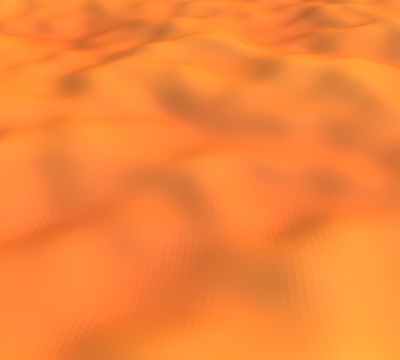
\includegraphics[scale=0.3]{smoothTerrain}
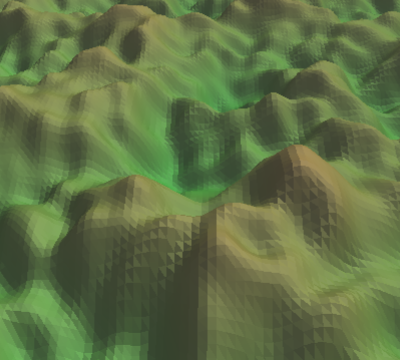
\includegraphics[scale=0.3]{unevenTerrain}
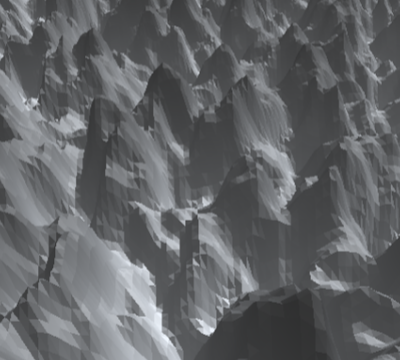
\includegraphics[scale=0.3]{roughTerrain}
\caption{Examples of the three terrain types. From left to right: Smooth, Uneven, Rough.}
\end{figure}\\
At one point the height of the terrain was proportional to the number of sections of the robot, a similar method to that of the Octopus robot. However, as the terrain is a control variable the heights were switched to a static value: $Smooth=8, Uneven=16, Rough=24$.\\
Overall, the rougher the terrain, the higher and more closed in it is. Most of the development of the robot was conducted on the smooth and uneven terrains, as the rough terrain aims to provide a more extreme environment with which to test the efficacy of the AI.\\
The smooth terrain is deliberately featureless to test the behaviour of the robot in a simple environment. Herbert Simon provided an elegant example of the importance of this consideration: an ant is observed making its way back to its nest across a beach.\\
Its route is ‘a sequence of irregular, angular segments’ that suggests some level of complexity in the ant's behaviour. However, the beach for the ant is a much harsher environment than it is for a human. It is more likely that ‘its complexity is really a complexity in the surface of the beach, not a complexity in the ant.’ Thus, the situatedness of the robot could culminate in behaviours that are not of its own making and are instead caused by its relationship with the terrain. The smooth terrain should reduce the role of the environment and allow for emergent behaviours to be prescribed to the robot itself. It is worth noting that the robot is still being tested on three terrains with some common properties (e.g. gravity) and these factors may introduce bias in the AI. This is a reasonable situation as long as applications of the Lizardbot are further modelled on encounterable terrains to allow the AI to adapt the robot accordingly. For proof of concept the sample set of terrains is sufficient.
\subsection{Body}
Insert from progress log \& CPG log\\
The velocity that should be applied to this section is calculated using\\\\
\begin{Large}
$\overrightarrow{v_{i}} = \overrightarrow{v_{i-1}} + \frac{m}{2}\overrightarrow{w} $\\\\
\end{Large}
For rotating sections $i = 0, ..., m$, where $m \leq n$, the value of $w$ will be calculated using $S$ or $C$ as specified.\\\\
\begin{Large}
$S: \overrightarrow{w} = sin\overrightarrow{\theta_{i-1}} + sin\overrightarrow{\theta_{i}}$\\\\
$C: \overrightarrow{w} = cos\overrightarrow{\theta_{i-1}} + cos\overrightarrow{\theta_{i}}$
\end{Large}
\subsection{Tail}
Insert from tail log\\
\begin{Large}\\
$r = |x_{i} - \frac{1}{n}\sum_{i}^{n}m_{i}x_{i}|$\\\\
$L = \sum^{n}_{i} r_{i}m_{i}v_{i}$\\\\
$v_{t} = - \frac{L}{r_{t}m_{t}}$
\end{Large}

\subsection{Legs}
\begin{Large}
$P = D + Vcos\theta + Ucos\theta$\\\\
$v_{i} = g(P_{i + 1} - P_{i})$
\end{Large}
\subsection{Performance}
Insert from trapped algorithm log - get performance from GA
\subsection{Genetic Algorithm}
Insert from GA log\\
\begin{Large}\\
$G_{i} = R^{[0, 1]} < m \longrightarrow 
(max(G_{i}) - min(G_{i})) R^{[0.01, 0.1]}  G_{i}$\\\\
$G(1)_{i} = R^{[0, 1]} < r \longrightarrow$ 
\begin{LARGE}
$^{R^{[0, 1]} < 0.5\longrightarrow G(1)_{i}} 
_{R^{[0, 1]} \geq 0.5 \longrightarrow G(2)_{i}}$\\\\
\end{LARGE}

\end{Large}
where R denotes a randomly generated number. G(1) refers to the input robot, whilst G(2) is the selected robot. For \textit{Triad} recombination G(2) is randomly chosen from either of the two selected robots, with equal probability.
\subsection{Dynamic Systems}
Insert from DST log


\newpage
\section{Results}
How does mutating the body / movement independently work?\\
How does the addition of the tail help?\\
How does initiating the body with a serpentine motion established affect the outcome?\\
What happens when the body is set as static?\\
What is the outcome when the legs are out of sync from the body?\\
Starting with defaults, what parameters does the AI mutate to? What is the corresponding behaviour for this?\\
Does the AI converge on the same parameters when started with different defaults?\\



\newpage
\section{Conclusion}

\newpage
\section{References}
\bibliography{References}
\newpage
\section{Appendices}
\subsection{Code of Conduct}





\end{document}